\chapter{Related work - Rastermap Vectorization}
Image segmentation has come a long way on images of normal everyday objects with DCNN. However, none of the reviewed papers use their networks on raster maps. Not a lot of work has been done in regards to vectorization of raster maps using neural networks, and the author only found one paper on the subject. However, there has been a fair amount of research done on other image analysis techniques.

\section{Non-artifical intelligence methods}

\subsection{Color image segmentation in historical topographic maps based on homogeneity}
\citet{Leyk2010} presents a color image segmentation of raster maps from the \nth{19} century suffering from poor quality with a clustering technique using the local image plane, frequency domain an color space. The goal of the color image segmentation is to reduce the color values to fit the original colors used when printing the map. The method managed to segment lines, symbols and areas that belong to different color layers, however, there were still some minor classification errors that had to be solved manually. Results from the color segmentation can be seen in \autoref{fig:leyk2010}. Note that the output is not vector data, but a raster image with a lower number of colors.

\begin{figure}[H]
    \centering
    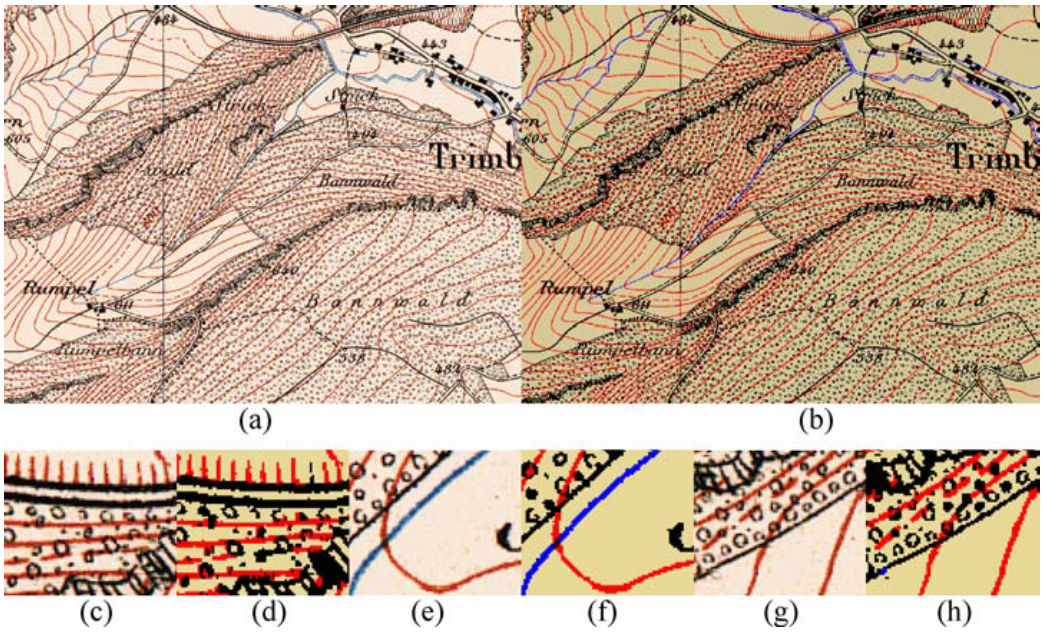
\includegraphics[width=0.8\linewidth]{fig/leyk2010.png}
    \captionsource{Color segmentation. (a) original map, (b) segmented map, (c-h) highlighted areas showing critical areas of the original.}{\citet{Leyk2010}}
    \label{fig:leyk2010}
\end{figure}

\subsection{Towards a comprehensive methodology for automatic vectorization of raster historical maps}
\citet{Iosifescu2016} use open-source solutions to vectorize historical maps from the \nth{19} century. Their procedure consists of five steps: Scanning of the map, georeferencing the map, pre-processing of the image to clean artifacts, automatic vectorization, automatic cleaning of the results. The authors note that the pre-processing step and scan quality are the most crucial for the performance of the vectorization and have to be customized for each set of raster maps. The pre-processing consist of RGB channel processing, conversion to binary images and cleaning. By processing the RGB channels in the image, different features on the map can be highlighted.

The pre-processed image is then converted to vector format with Geospatial Data Abstraction Library \cite{OSGeoa} (GDAL)'s polygonize and contour methods. The results are acceptable when taking the quality of the maps into consideration as seen in \autoref{fig:iosifescu2016}. 

\begin{figure}[H]
    \centering
    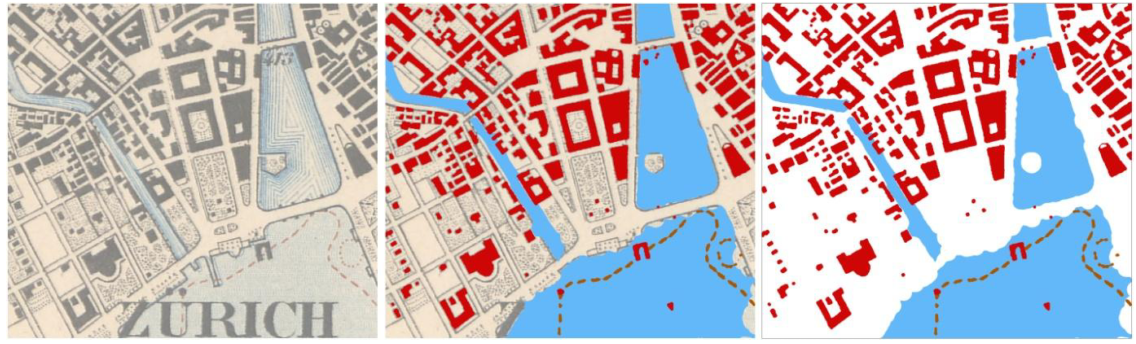
\includegraphics[width=0.9\linewidth]{fig/iosifescu2016.png}
    \captionsource{The final result of the vectorization of buildings, rivers and contours.}{\citet{Iosifescu2016}}
    \label{fig:iosifescu2016}
\end{figure}

\subsection{Historical map polygon and feature extractor}

\citet{GiraldoArteaga2013} vectorize polygons from old historical maps of building footprints in New York by using a procedure consisting of multiple open source tools. The tools in use are: GDAL \cite{OSGeoa}, OpenCV \cite{OpenVCTeam2017}, GIMP \cite{GIMP2017}, R \cite{TheRFoundation2017} and ImageMagic \cite{ImageMagickStudioLLC2017}. They propose a process consisting of three main steps: Raster image thresholding, rough polygon extraction and polygon analysis and simplification. There is a manual configuration step for each uniform set of map sheets where one has to enumerate the distinct colors in the map. The maps they are working on in the paper look very similar and therefore they only need to do this process one time for all the sheets. The input rasters can be seen in \autoref{fig:nyplmap} where we also see the result obtained from the process.

They state that the results will decrease the time spent on vectorizing the maps, but that the results do contain errors. These errors they propose to solve via crowd-sourcing tools.


\begin{figure}[H]
    \centering
    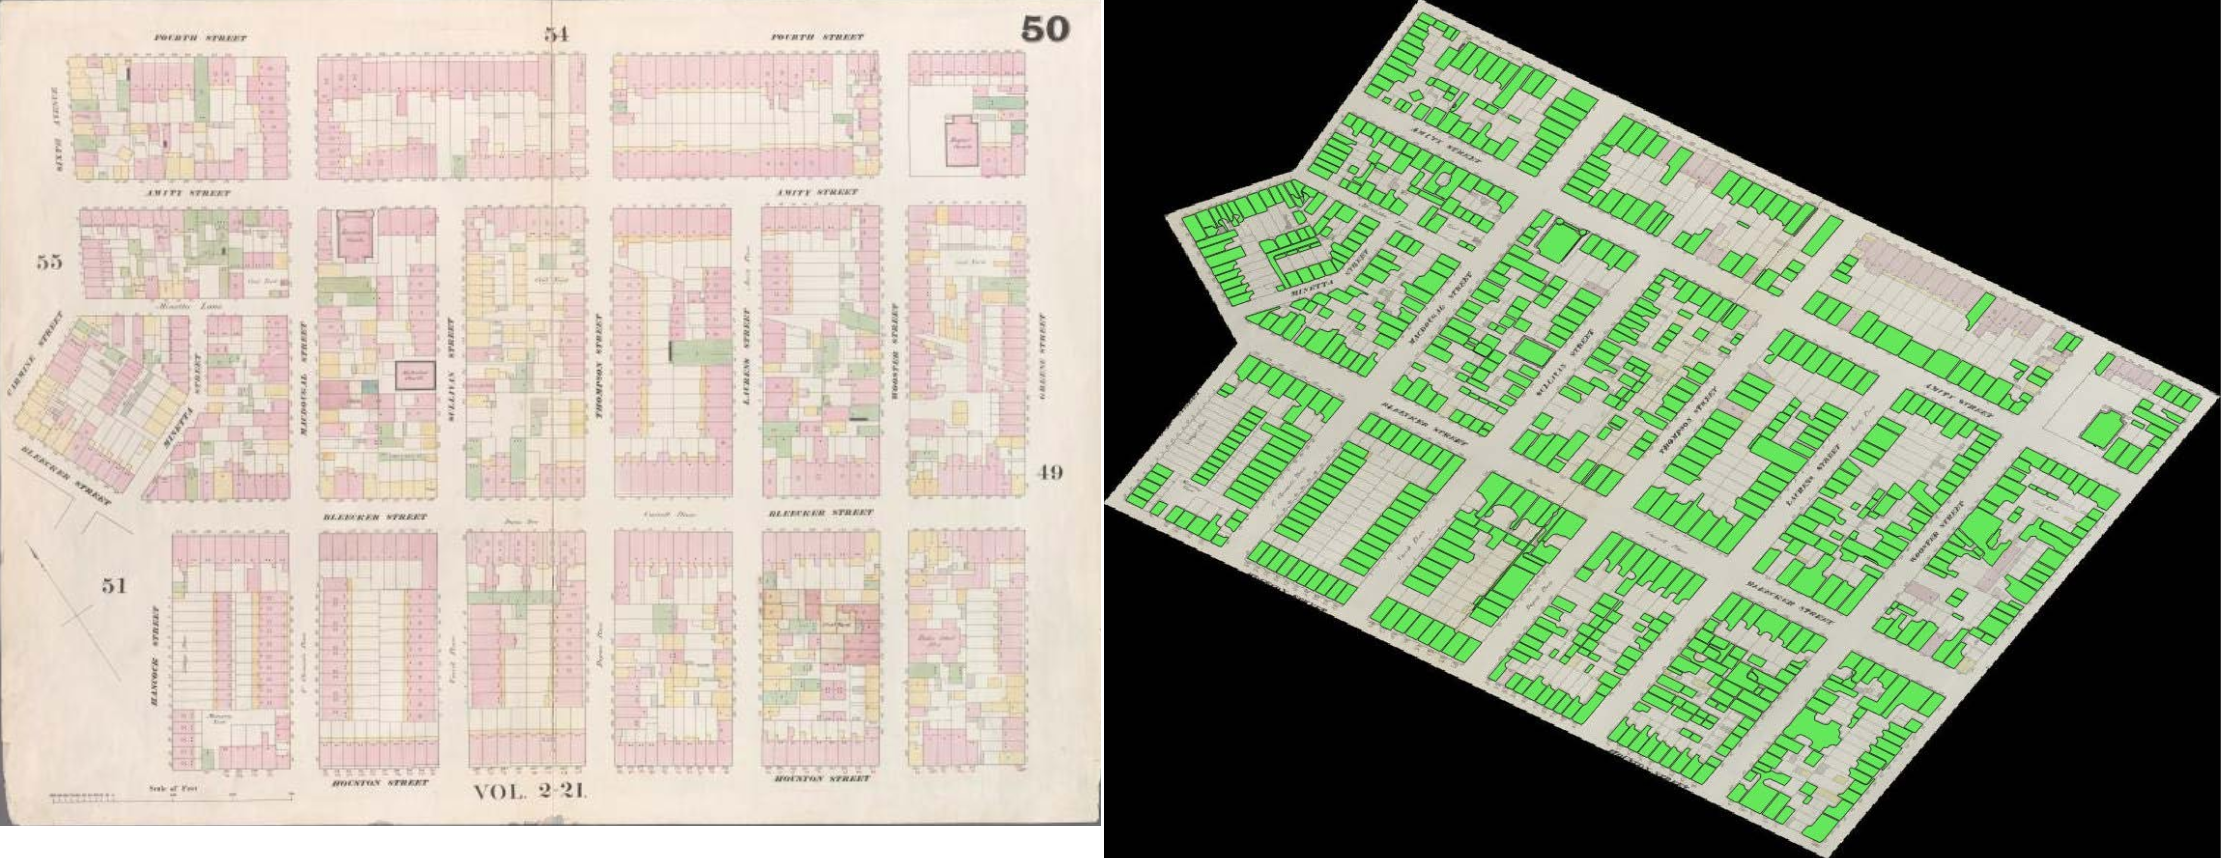
\includegraphics[width=\linewidth]{fig/nyplmap.png}
    \captionsource{Left: Input maps. Right: Output from the process}{\citet{GiraldoArteaga2013}}
    \label{fig:nyplmap}
\end{figure}

\subsection{A general approach for extracting road vector data from raster maps}

\citet{Chiang2013} present a semi-automatic technique for road extraction from raster maps with a system they call \emph{Strabo}. The system consists of two components: Road layer extraction and road layer vectorization. In their components, they use techniques such as mean-shift, k-means and Hough Transform. They compare they systems performance against R2V \cite{Wu1999}. Strabo performed better in 58.3\% of the cases. Generally, their road vector lines manage to stay in the center of the roads more than R2V. This can also be seen in \autoref{fig:chiang2013}. A limit of their system is that it struggles to correctly label roads that are very thin on the map. Their technique works on multiple different types of maps. 

\begin{figure}[H]
    \centering
    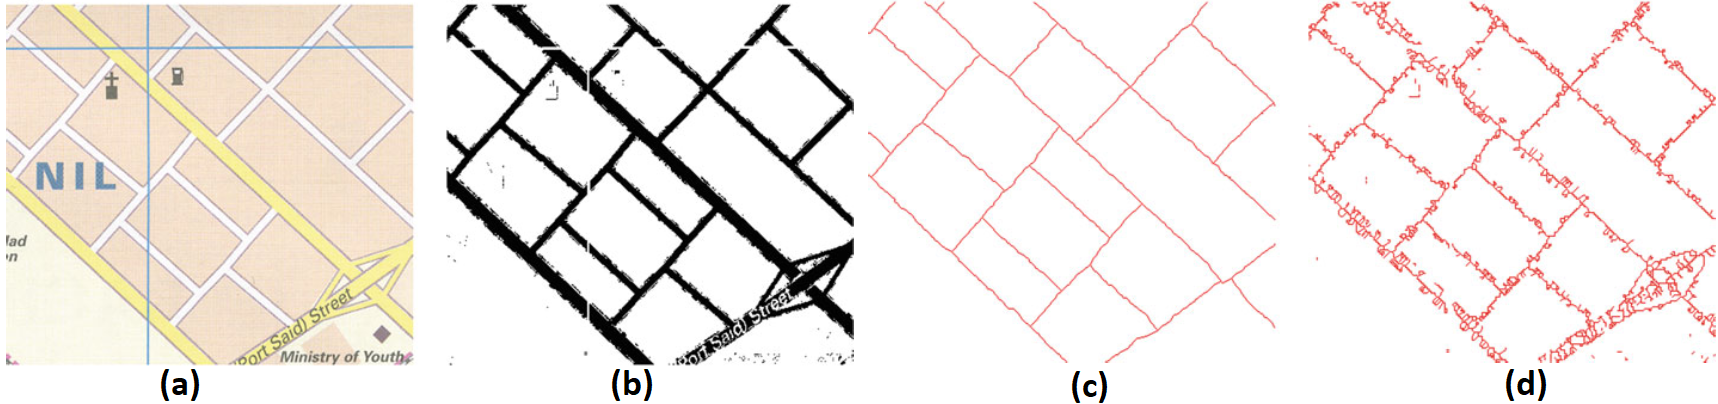
\includegraphics[width=0.9\linewidth]{fig/chiang2013.png}
    \captionsource{Vectorization results. (a) input map, (b) extracted road pixels, (c) Strabo results, (d) R2V results.}{\citet{Chiang2013}}
    \label{fig:chiang2013}
\end{figure}

\subsection{Guided Superpixel Method for Topographic Map Processing}
\citet{Miao2016} propose a \emph{superpixel}\cite{Ren2003} approach to extract height curves from raster maps. Their method, named \emph{Guided Superpixel Method in Topographic Map}(GSM-TM), consists of three parts: Linear feature extraction, boundary detection, and guided watershed transform. For the linear feature extraction, they merge two negative and two positive Gaussian filters. For the boundary extraction, they use a technique of color boundary detection proposed by \citet{Yang2013}. The guided watershed transform was introduced since standard watershed is very sensitive to weak boundaries. The guided part consist of modifying the boundaries obtained in the boundary detection step with the lines obtained in the linear feature extraction to make the boundaries clearer before the watershed transform. The results show that the proposed GSM-TM method performs better than the other superpixel algorithms they compare with, also seen in \autoref{fig:miao2016}. 

\begin{figure}[H]
    \centering
    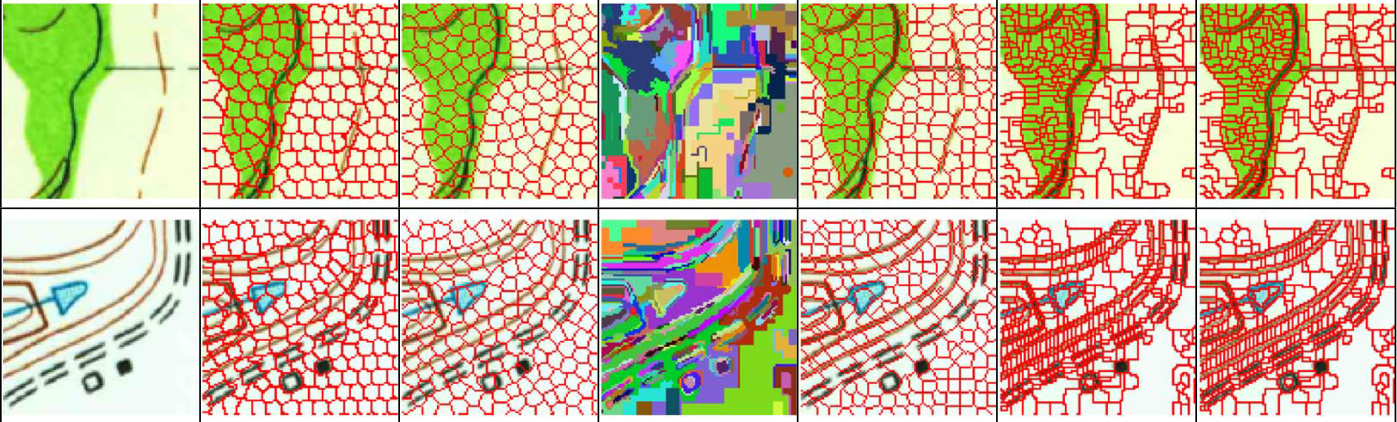
\includegraphics[width=0.9\linewidth]{fig/miao2016.png}
    \captionsource{Results of compared methods. From left to right are the original map and the results from SLIC, NC, GS, Turbopixel, WT and GSM-TM}{\citet{Miao2016}}
    \label{fig:miao2016}
\end{figure}

\section{Artificial intelligence methods}

\subsection{VecNET}
VecNet proposed by \citet{Karabork2008} in 2008 is one of few examples of vectorization of cartographic raster maps using a neural network. The authors present a three-step process consisting of thinning, line tracking with ANN and simplification. The main goal of the network is to find the critical points of objects, that is, to find breakage points of lines. They use an ANN with an input layer, a hidden layer and an output layer to classify. The training set is very small with only 16 samples. The output layer is a single vector with size 12, where the 8 first places represent an 8-way chain code of directions (the direction the line is following) and the last four represent a prediction of where the next pixel is going to be. It evaluates if the point is critical by checking if the last 8-way direction is different from the one currently calculated. If the point is critical, they store it. The algorithm is tested on a single raster map only consisting of lines and does not perform better than sparse pixel SPV, but manages to get acceptable results. 
